\documentclass{article}

\usepackage{geometry}
\usepackage{amsmath}
\usepackage{graphicx}
\usepackage{listings}
\usepackage{hyperref}
\usepackage{multicol}
\usepackage{fancyhdr}
\usepackage{enumerate}
\pagestyle{fancy}
\hypersetup{ colorlinks=true, linkcolor=black, filecolor=magenta, urlcolor=cyan}
\geometry{ a4paper, total={170mm,257mm}, top=20mm, right=20mm, bottom=20mm, left=20mm}
\setlength{\parindent}{0pt}
\setlength{\parskip}{1em}
\renewcommand{\headrulewidth}{0pt}
\lhead{Competitive Programming - Arkavidia V}
\fancyfoot[CE,CO]{J - \thepage}
\lstset{
    basicstyle=\ttfamily\small,
    columns=fixed,
    extendedchars=true,
    breaklines=true,
    tabsize=2,
    prebreak=\raisebox{0ex}[0ex][0ex]{\ensuremath{\hookleftarrow}},
    frame=none,
    showtabs=false,
    showspaces=false,
    showstringspaces=false,
    prebreak={},
    keywordstyle=\color[rgb]{0.627,0.126,0.941},
    commentstyle=\color[rgb]{0.133,0.545,0.133},
    stringstyle=\color[rgb]{01,0,0},
    captionpos=t,
    escapeinside={(\%}{\%)}
}

\begin{document}

\begin{center}
    \section*{J. Jalur kereta}

    \begin{tabular}{ | c c | }
        \hline
        Batas Waktu  & 1s \\
        Batas Memori & 512MB \\
        \hline
    \end{tabular}
\end{center}

\subsection*{Deskripsi}

Negeri Ganesha memiliki peta jalur kereta yang terdiri dari banyak jalur kereta, menghubungkan kota A dan kota B.
Peta jalur kereta ini sangat rumit, sehingga peta jalur kereta ini hanya boleh dilewati oleh kereta dari kota A ke B, tidak sebaliknya.
Lalu, \textbf{hanya ada satu} jalur kereta yang keluar dari kota A dan \textbf{hanya ada satu} jalur kereta yang masuk ke kota B.

\begin{multicols}{2}
\begin{center}
    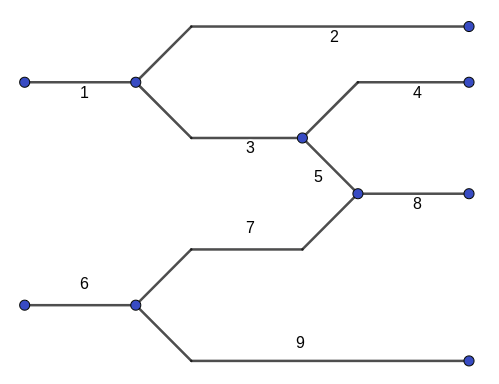
\includegraphics[width=200px]{sample-1}
\end{center}

Di samping ini merupakan contoh peta jalur kereta yang terdiri dari 10 jalur kereta (kiri adalah kota A dan kanan adalah kota B).
Hanya terdapat 2 jenis persimpangan, yakni:
\begin{enumerate}[A.]
    \setlength{\itemsep}{0pt}
    \item Sebuah jalur terbagi menjadi dua jalur berbeda
    \item Dua jalur berbeda bergabung menjadi satu jalur
\end{enumerate}
\end{multicols}

Sebagai contoh, persimpangan di ujung akhir jalur 1 merupakan persimpangan jenis A dan persimpangan di ujung awal jalur 6 merupakan persimpangan jenis B.
Sudah dipastikan tidak ada dua jalur yang saling tumpang tindih.
Selain itu, jalur yang langsung keluar dari kota A pasti bernomor 1 dan jalur yang langsung masuk ke kota B pasti bernomor paling besar.

Menurut Arvy, penempatan dua kereta di jalur $x$ dan $y$ dianggap bagus jika $x$ tidak bisa dicapai dari $y$ dan $y$ tidak bisa dicapai dari $x$ (ingat kalau semua rel hanya satu arah, dari kiri ke kanan).
Kini ia bertanya, berapa maksimum kereta yang bisa ditempatkan sehingga penempatan \textbf{setiap} dua pasang kereta dianggap bagus oleh Arvy.

\subsection*{Format Masukan}
Baris pertama terdiri dari satu bilangan bulat positif $T$ ($1 \leq T \leq 10$), menyatakan banyaknya kasus uji.
Setiap kasus uji diawali dengan bilangan $N$ ($1 \leq N \leq 100.000$) menyatakan banyaknya persimpangan dan banyaknya jalur.
$N$ baris berikutnya memiliki format:
\begin{itemize}
    \setlength{\itemsep}{0pt}
    \item \lstinline{A a b c}, menandakan adanya persimpangan tipe A, yakni jalur nomor \lstinline{a} bercabang menjadi \lstinline{b} dan \lstinline{c} (dari jalur \lstinline{a}, belok kiri untuk ke jalur \lstinline{b} atau belok kanan untuk ke jalur \lstinline{c}).
    \item \lstinline{B a b c}, menandakan adanya persimpangan tipe B, yakni jalur nomor \lstinline{a} dan \lstinline{b} bergabung menjadi \lstinline{c} (jalur \lstinline{a} berada di kiri jalur \lstinline{b}).
\end{itemize}

\subsection*{Format Keluaran}
Untuk setiap kasus uji, tuliskan dalam satu baris, banyaknya kereta maksimum yang dapat ditempatkan sehingga penempatan tiap dua pasang kereta dianggap bagus oleh Arvy.

\pagebreak

\begin{multicols}{2}
\subsection*{Contoh Masukan}
\begin{lstlisting}
1
6
A 1 2 3
A 2 4 5
B 4 7 6
A 3 7 8
B 5 6 9
B 9 8 10
\end{lstlisting}
\columnbreak
\subsection*{Contoh Keluaran}
\begin{lstlisting}
4
\end{lstlisting}
\vfill
\null
\end{multicols}

\subsection*{Penjelasan}
Pada kasus uji pertama, peta jalur kereta dapat digambarkan seperti peta yang ada di deskripsi soal. Penempatan yang maksimum salah satunya dengan menempatkan kereta pada nomor $4$, $5$, $7$, dan $8$.

\end{document}
